\begin{enumerate}[label=\thechapter.\arabic*,ref=\thechapter.\theenumi]
\item The network shown below has a resonant frequency of 150 kHz and bandwidth of 600
Hz. The Q-factor of the network is \rule{1cm}{0.15mm}\\
(rounded off to one decimal place).\\
\hfill(GATE 2022 EC)\\
\begin{figure}[ht]
  \centering
  
      \begin{circuitikz}[american]
    \draw (0,0) to [short, *-] (5,0) to [R=R] (5,2) to [L=L] (5,4) to [short] (2,4) to [C=C] (2,0);
    \draw (0,4) to [short, *-] (2,4);
\end{circuitikz}
  
  \caption{Circuit 1}
\end{figure}\\
\solution\\
\iffalse
\documentclass[journal,12pt,twocolumn]{IEEEtran}
\usepackage{amsmath,amssymb,amsfonts,amsthm}
\usepackage{txfonts}
\usepackage{tkz-euclide}
\usepackage{listings}
\usepackage{gvv}
\usepackage[latin1]{inputenc}
\usepackage{adjustbox}
\usepackage{array}
\usepackage{tabularx}
\usepackage{enumitem}
\usepackage{pgf}
\usepackage{lmodern}
\usepackage{circuitikz}
\usepackage{tikz}
\usepackage{graphicx}


\begin{document}
\bibliographystyle{IEEEtran}

\vspace{3cm}

\title{}
\author{EE23BTECH11054 -  Sai Krishna Shanigarapu$^{*}$
}
\maketitle
\newpage
\bigskip

\section*{Gate EE 2022}
28. \hspace{2pt}The network shown below has a resonant frequency of 150 kHz and bandwidth of 600
Hz. The Q-factor of the network is \rule{1cm}{0.15mm}\\
(rounded off to one decimal place).\\
\hfill(GATE 2022 EC)\\
\begin{figure}[ht]
  \centering
  
      \begin{circuitikz}[american]
    \draw (0,0) to [short, *-] (5,0) to [R=R] (5,2) to [L=L] (5,4) to [short] (2,4) to [C=C] (2,0);
    \draw (0,4) to [short, *-] (2,4);
\end{circuitikz}
  
  \caption{Circuit 1}
\end{figure}\\
\solution
\fi

\begin{figure}[ht]
  \centering
  
      \begin{circuitikz}[american]
    \draw (0,0) to [short, *-] (5,0) to [R=R] (5,2) to [L=$j\omega L$] (5,4) to [short] (2,4) to [C=$\frac{1}{j\omega C}$] (2,0);
    \draw (0,4) to [short, *-] (2,4);
\end{circuitikz}

  \caption{Circuit 2}
\end{figure}


\begin{table}[ht]
    \centering
 
    \setlength{\arrayrulewidth}{0.3mm}
\setlength{\tabcolsep}{20pt}
\renewcommand{\arraystretch}{1.3}


\begin{tabular}{|c|c|c|}
\hline
Parameter & Description & Value\\
\hline
$f_0$ & Resonant frequency & 150 kHz\\
\hline
$B$ & Bandwidth & 600 Hz\\
\hline
\end{tabular}

    \caption{Parameters}
    \label{tab:tab1_gate_ee_2022_28_054}
\end{table}

\begin{table}[ht]
    \centering

    \setlength{\arrayrulewidth}{0.3mm}
\setlength{\tabcolsep}{20pt}
\renewcommand{\arraystretch}{1.5}


\begin{tabular}{|c|c|c|}
\hline
Parameter & Description & Formula\\
\hline
$Q$ & Quality factor & $\frac{X_L}{R}$\\
\hline
$B$ & Bandwidth & $\frac{R}{2 \pi L}$\\
\hline
$\omega_0$ & Radial resonant frequency & $2 \pi f_0$\\
\hline
$X_L$ & Inductive reactance & $\omega L$\\
\hline
$X_C$ & Capacitive reactance & $\frac{1}{\omega C}$\\
\hline

\end{tabular}


    \caption{Formulae}
    \label{tab:tab2_gate_ee_2022_28_054}
\end{table}

At Resonance, 
\begin{align}
    X_L & = X_C\\
    \omega_0 L &= \frac{1}{\omega_0 C}\\
    \omega_0 &= \frac{1}{\sqrt{LC}}\\
    2 \pi f_0 &= \frac{1}{\sqrt{LC}}\\
    \implies f_0 &= \frac{1}{2 \pi \sqrt{LC}} \label{eq:eq1_gate_ee_2022_28_054}    
\end{align}

Using Table \ref{tab:tab2_gate_ee_2022_28_054},
\begin{align}
    Q &= \frac{X_L}{R}\\
    &= \frac{\omega_0 L}{R}\\
    &= \brak{\frac{1}{\sqrt{LC}}}\frac{L}{R}\\
    \implies Q &= \frac{1}{R}\sqrt{\frac{L}{C}} \label{eq:eq2_gate_ee_2022_28_054}
\end{align}

From eq (\ref{eq:eq1_gate_ee_2022_28_054}) and Table \ref{tab:tab2_gate_ee_2022_28_054}
\begin{align}
    \frac{f_0}{B} &= \brak{\frac{1}{2\pi \sqrt{LC}}}\frac{2 \pi L}{R}\\
    &= \brak{\frac{1}{\sqrt{LC}}}\frac{L}{R}\\
    \implies \frac{f_0}{B} &= \frac{1}{R}\sqrt{\frac{L}{C}} \label{eq:eq3_gate_ee_2022_28_054}
\end{align}

From Table \ref{tab:tab1_gate_ee_2022_28_054}, eq (\ref{eq:eq2_gate_ee_2022_28_054}) and eq (\ref{eq:eq3_gate_ee_2022_28_054}),
\begin{align}
    Q &= \frac{f_0}{B}\\
     &=\frac{150 \text{ x } 10^3}{600}\\
    &= 250
\end{align}

$\therefore$ Q-factor is 250

\begin{figure}[ht]
    \centering
    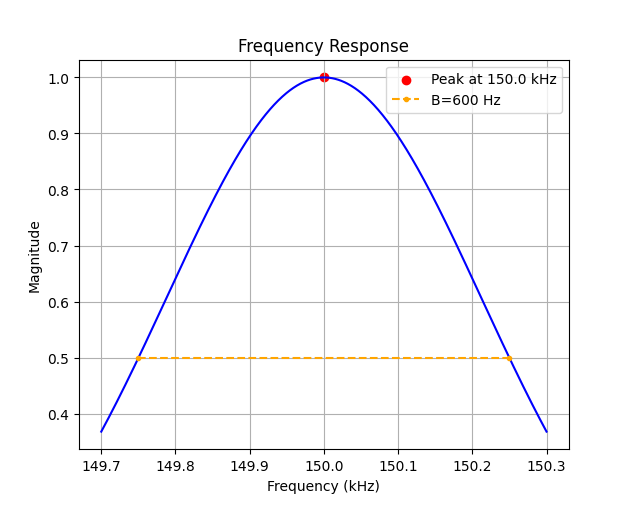
\includegraphics[width=\columnwidth]{2022/EE/28/figs/Figure_1.png}
    \caption{Plot of Q-factor}
    \label{fig:fig1_gate_ee_2022_18_054}
\end{figure}

%\end{document}

\pagebreak

\item In the circuit shown below, the switch S is closed at $t=0$. The magnitude of the steady state voltage, in volts, across the $6\Omega$ resistor is \_\_\_\_\_.(\textit{round off to two decimal places})\\ \hfill(GATE 2022 EE Q31)
\begin{figure}[!h]
    \centering
    \begin{circuitikz}[scale = 0.8]
        \draw(0, 0) -- (1, 0);
        \draw(1, 0.5) -- (1, -0.5);
        \draw(4, 0.5) -- (4, -0.5);
        \draw(4, 0) -- (5, 0);

        \draw(1, 0.5) to[R, l = $6\Omega$](4, 0.5);
        \draw(1, -0.5) to[R, l_ = $3\Omega$](4, -0.5);

        \draw(0, 0) -- (0, -2);
        \draw(5, 0) -- (5, -2);

        \draw(0, -2) to[C, l = $1\mu F$](2, -2);
        \draw(2, -2) to [R, l = $10\Omega$](5, -2);

        \draw(0, -2) -- (0, -3.5);
        \draw(5, -2) -- (5, -3.5);

        \draw(0, -3.5) to[battery2, l_ = $10V$](1.5, -3.5);
        \draw (1.5, -3.5) to[switch, l = S] (2, -3.5);
        \draw(2, -3.5) to [R, l = $2\Omega$](5, -3.5);

        \draw[->](0, -3.5) -- (0, -2.5) node[midway, left] {$I$}; 
    \end{circuitikz}
    \caption{}
    \label{fig:1_gate.ee.22.31}
\end{figure}\\
\solution
		\iffalse
\let\negmedspace\undefined
\let\negthickspace\undefined
\documentclass[journal,12pt,twocolumn]{IEEEtran}
\usepackage{cite}
\usepackage{amsmath,amssymb,amsfonts,amsthm}
\usepackage{algorithmic}
\usepackage{graphicx}
\usepackage{textcomp}
\usepackage{xcolor}
\usepackage{txfonts}
\usepackage{listings}
\usepackage{enumitem}
\usepackage{mathtools}
\usepackage{gensymb}
\usepackage{comment}
\usepackage[breaklinks=true]{hyperref}
\usepackage{tkz-euclide} 
\usepackage{listings}
\usepackage{gvv}                            \usepackage{tikz}
\usepackage{circuitikz}
\def\inputGnumericTable{}                                
\usepackage[latin1]{inputenc}                            
\usepackage{color}                                       
\usepackage{array}                                       
\usepackage{longtable}                                   
\usepackage{calc}                              
\usepackage{tikz}
\usepackage{multirow}                                    
\usepackage{hhline}                                      
\usepackage{ifthen}                            
\usepackage{caption}
\usepackage{lscape}
\usepackage{amsmath}
\newtheorem{theorem}{Theorem}[section]
\newtheorem{problem}{Problem}
\newtheorem{proposition}{Proposition}[section]
\newtheorem{lemma}{Lemma}[section]
\newtheorem{corollary}[theorem]{Corollary}
\newtheorem{example}{Example}[section]
\newtheorem{definition}[problem]{Definition}
\newcommand{\BEQA}{\begin{eqnarray}}
\newcommand{\EEQA}{\end{eqnarray}}
\newcommand{\define}{\stackrel{\triangle}{=}}
\theoremstyle{remark}
\newtheorem{rem}{Remark}

\begin{document}

\bibliographystyle{IEEEtran}
\vspace{3cm}

\title{GATE 2023 PH Q37}
\author{EE23BTECH11009 - AROSHISH PRADHAN$^{*}$% <-this % stops a space
}
\maketitle
\newpage
\bigskip
\textbf{Question:} In the circuit shown below, the switch S is closed at $t=0$. The magnitude of the steady state voltage, in volts, across the $6\Omega$ resistor is \_\_\_\_\_.(\textit{round off to two decimal places})\\ \hfill(GATE 2022 EE Q31)
\begin{figure}[!h]
    \centering
    \begin{circuitikz}[scale = 0.8]
        \draw(0, 0) -- (1, 0);
        \draw(1, 0.5) -- (1, -0.5);
        \draw(4, 0.5) -- (4, -0.5);
        \draw(4, 0) -- (5, 0);

        \draw(1, 0.5) to[R, l = $6\Omega$](4, 0.5);
        \draw(1, -0.5) to[R, l_ = $3\Omega$](4, -0.5);

        \draw(0, 0) -- (0, -2);
        \draw(5, 0) -- (5, -2);

        \draw(0, -2) to[C, l = $1\mu F$](2, -2);
        \draw(2, -2) to [R, l = $10\Omega$](5, -2);

        \draw(0, -2) -- (0, -3.5);
        \draw(5, -2) -- (5, -3.5);

        \draw(0, -3.5) to[battery2, l_ = $10V$](1.5, -3.5);
        \draw (1.5, -3.5) to[switch, l = S] (2, -3.5);
        \draw(2, -3.5) to [R, l = $2\Omega$](5, -3.5);

        \draw[->](0, -3.5) -- (0, -2.5) node[midway, left] {$I$}; 
    \end{circuitikz}
    \caption{}
    \label{fig:1_gate.ee.22.31}
\end{figure}\\

\solution 
\fi
Consider a sinusoidal input source of angular frequency $\omega$.

\begin{table}[!h]
    \centering
    \begin{tabular}{|c|c|c|}
    \hline
       \textbf{Symbol}  &  \textbf{Value}  &  \textbf{Description}\\
    \hline
       $\omega$  &  $0$ for D.C. &  Angular Frequency\\
    \hline
        $C$ & $1\mu F$ & Capacitance \\
    \hline
        $V_{in}(t)$ & $10\cos(\omega t)$ & Input Voltage\\
    \hline
        $V_{out}(t)$ &  & Output Voltage across $6\Omega$\\
    \hline
        $V_{out}(j\omega)$ & $H(j\omega)V_{in}(j\omega)$ & Output in Frequency Domain\\
    \hline
        $H(j\omega)$ &  & Transfer Function\\
    \hline
        $I(j\omega)$ & & Total Current\\
    \hline
        $Z_{\text{eff}}$ & & Overall Impedance\\
    \hline
    \end{tabular}
    \caption{Given Parameters}
    \label{tab:1_gate.22.ee.31}
\end{table}

Using KCL and KVL, we can calculate:
\begin{align}
    Z_{\text{eff}} &= \frac{2\brak{10 + \frac{1}{j\omega C}}}{12 + \frac{1}{j\omega C}} + 2\\
    \implies I(j\omega) &= \frac{V_{in}}{\brak{\frac{2\brak{10 + \frac{1}{j\omega C}}}{12 + \frac{1}{j \omega C}}+2}}\\
    \implies V_{out}(j\omega) &= 2\sbrak{\brak{\frac{10 + \frac{1}{j\omega C}}{12 + \frac{1}{j\omega C}}}I(j\omega)}\\
    &= 2\sbrak{\brak{\frac{10 + \frac{1}{j\omega C}}{12 + \frac{1}{j\omega C}}}\frac{V_{in}(j\omega)}{\brak{\frac{2\brak{10 + \frac{1}{j\omega C}}}{12 + \frac{1}{j \omega C}}+2}}}\\
    \implies H(j\omega) &= \frac{1 + 10j\omega C}{2(1 + 11j\omega C)}
\end{align}
\begin{figure}[!h]
    \centering
    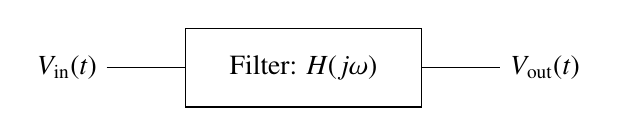
\begin{tikzpicture}
    % Draw the filter rectangle
    \draw (0,0) rectangle (3,1) node[midway] {Filter: $H(j\omega)$};
    
    % Draw the input and output labels
    \draw (-1,0.5) node[left] {$V_{\text{in}}(t)$} -- (0,0.5);
    \draw (3,0.5) -- (4,0.5) node[right] {$V_{\text{out}}(t)$};
\end{tikzpicture}
    \caption{Filter Equivalent of Circuit}
    \label{fig:2_gate.22.ee.31}
\end{figure}
\begin{align}
    H(j\omega) &= \brak{\frac{\sqrt{1 + 100\omega^2 C^2}}{2\sqrt{1 + 121\omega^2 C^2}}}e^{j(\tan^{-1}(10\omega C) - \tan^{-1}(11\omega C))}\\
    &= \brak{\frac{\sqrt{1 + 100\omega^2 C^2}}{2\sqrt{1 + 121\omega^2 C^2}}}e^{j\tan^{-1}\brak{\frac{-\omega C}{1 + 110\omega^2 C^2}}}\\
    \therefore V_{out}(t) &= 10\abs{H(j\omega)}\cos(\omega t + \angle H(j\omega))\\
    &= \frac{5\sqrt{1 + 100\omega^2 C^2}}{\sqrt{1 + 121\omega^2 C^2}}\cos\brak{\omega t -\tan^{-1}\brak{\frac{\omega C}{1 + 110\omega^2 C^2}}}
\end{align}
\begin{figure}[!h]
    \centering
    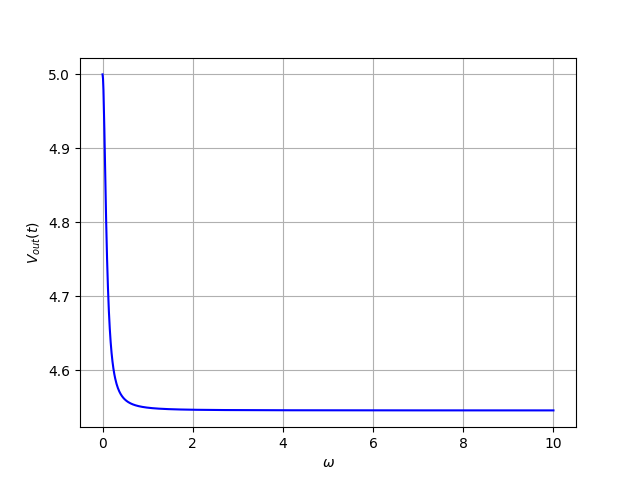
\includegraphics[width = \columnwidth]{2022/EE/31/figs/V_out_plot.png}
    \caption{Plot of $V_{out}(t)$ at $t=0$ w.r.t $\omega$}
    \label{fig:3_gate.22.ee.31}
\end{figure}

As $\omega \rightarrow 0$, $V_{in}(t)$ approaches being a D.C. input source ($10V$).

$\therefore$ substituting $\omega = 0$, we get:
\begin{align}
    V_{out}(t) &= 5V
\end{align}

%\end{document}


\pagebreak

\item In the circuit shown, the load is driven by a sinusoidal A.C. voltage source $V_1 = 100\angle0\degree V$ at $50Hz$. Given $R_1 = 20\Omega$, $C_1 = \brak{\frac{1000}{\pi}}\mu F$, $L_1 = \brak{\frac{20}{\pi}}mH$ and $R_2 = 4\Omega$, the power factor is \_\_\_\_\_ (round off to one decimal place)\\
\hfill(GATE 2022 IN Q52)
\begin{figure}[!h]
    \centering
    \begin{circuitikz}
        \draw(0, 0) to[sV, l = $V_1$](0, -4);
        \draw(0, -4) to [R, l = $R_2$](6, -4);
        \draw(6, 0) to[L, l = $L_1$](6, -4);
        \draw(0, 0) -- (2, 0);
        \draw(4, 0) -- (6, 0);
        \draw(2, 0.75) -- (2, -0.75);
        \draw(4, 0.75) -- (4, -0.75);

        \draw(2, 0.75) to [R, l = $R_1$](4, 0.75);
        \draw(2, -0.75) to [C, l_ = $C_1$](4, -0.75);
    \end{circuitikz}
    \caption{}
    \label{fig:1_gate.22.in.52}
\end{figure}

\solution
		\iffalse
\let\negmedspace\undefined
\let\negthickspace\undefined
\documentclass[journal,12pt,twocolumn]{IEEEtran}
\usepackage{cite}
\usepackage{amsmath,amssymb,amsfonts,amsthm}
\usepackage{algorithmic}
\usepackage{graphicx}
\usepackage{textcomp}
\usepackage{xcolor}
\usepackage{txfonts}
\usepackage{listings}
\usepackage{enumitem}
\usepackage{mathtools}
\usepackage{gensymb}
\usepackage{comment}
\usepackage[breaklinks=true]{hyperref}
\usepackage{tkz-euclide} 
\usepackage{listings}
\usepackage{gvv}                            \usepackage{tikz}
\usepackage{circuitikz}
\def\inputGnumericTable{}                                
\usepackage[latin1]{inputenc}                            
\usepackage{color}                      \usepackage{gensymb}
\usepackage{array}                                       
\usepackage{longtable}                                   
\usepackage{calc}                              
\usepackage{tikz}
\usepackage{multirow}                                    
\usepackage{hhline}                                      
\usepackage{ifthen}                            
\usepackage{caption}
\usepackage{lscape}
\usepackage{amsmath}
\newtheorem{theorem}{Theorem}[section]
\newtheorem{problem}{Problem}
\newtheorem{proposition}{Proposition}[section]
\newtheorem{lemma}{Lemma}[section]
\newtheorem{corollary}[theorem]{Corollary}
\newtheorem{example}{Example}[section]
\newtheorem{definition}[problem]{Definition}
\newcommand{\BEQA}{\begin{eqnarray}}
\newcommand{\EEQA}{\end{eqnarray}}
\newcommand{\define}{\stackrel{\triangle}{=}}
\theoremstyle{remark}
\newtheorem{rem}{Remark}

\begin{document}

\bibliographystyle{IEEEtran}
\vspace{3cm}

\title{GATE 2022 IN Q52}
\author{EE23BTECH11009 - AROSHISH PRADHAN$^{*}$% <-this % stops a space
}
\maketitle
\newpage
\bigskip
\textbf{Question:} In the circuit shown, the load is driven by a sinusoidal A.C. voltage source $V_1 = 100\angle0\degree V$ at $50Hz$. Given $R_1 = 20\Omega$, $C_1 = \brak{\frac{1000}{\pi}}\mu F$, $L_1 = \brak{\frac{20}{\pi}}mH$ and $R_2 = 4\Omega$, the power factor is \_\_\_\_\_ (round off to one decimal place)\\
\hfill(GATE 2022 IN Q52)
\begin{figure}[!h]
    \centering
    \begin{circuitikz}
        \draw(0, 0) to[sV, l = $V_1$](0, -4);
        \draw(0, -4) to [R, l = $R_2$](6, -4);
        \draw(6, 0) to[L, l = $L_1$](6, -4);
        \draw(0, 0) -- (2, 0);
        \draw(4, 0) -- (6, 0);
        \draw(2, 0.75) -- (2, -0.75);
        \draw(4, 0.75) -- (4, -0.75);

        \draw(2, 0.75) to [R, l = $R_1$](4, 0.75);
        \draw(2, -0.75) to [C, l_ = $C_1$](4, -0.75);
    \end{circuitikz}
    \caption{}
    \label{fig:1_gate.22.in.52}
\end{figure}


\solution
\fi
\begin{table}[!h]
    \centering
    \begin{tabular}{|c|c|c|}
    \hline
       \textbf{Symbol}  & \textbf{Value}  & \textbf{Description}\\
    \hline
       $V_1$  & $100\angle0\degree V$ & Input Voltage \\
    \hline
        $f$ & $50Hz$ & Frequency\\
    \hline
        $\omega$ & $2\pi f$ & Angular Frequency\\
    \hline
        $R_1$ & $20\Omega$ & Resistance\\
    \hline
        $R_2$ & $4\Omega$ & Resistance\\
    \hline
        $C_1$ & $\brak{\frac{1000}{\pi}}\mu F$ & Capacitance\\
    \hline
        $L_1$ & $\brak{\frac{20}{\pi}}mH$ & Inductance\\
    \hline
        $Z_{\text{eff}}$ & & Impedance\\
    \hline
        $\cos(\phi)$ & $\dfrac{\mathrm{Re}(Z_{\text{eff}})}{\abs{Z_{\text{eff}}}}$& Power Factor\\
    \hline
    \end{tabular}
    \caption{Given Parameters}
    \label{tab:1_gate.22.in.52}
\end{table}


\begin{align}
    Z_{\text{eff}} &= R_2 + j\omega L_1 + \frac{\frac{R_1}{j\omega C_1}}{R_1 + \frac{1}{j\omega C_1}}\\
    &= 4 + 2j + \frac{-200j}{20 - 10j}\\
    &= 8-6j
\end{align}
$\therefore$ Power Factor:
\begin{align}
    \cos(\phi) &= \frac{\mathrm{Re}(Z_{\text{eff}})}{\abs{Z_{\text{eff}}}}\\
    &= \frac{8}{\sqrt{8^2 + 6^2}}\\
    &= 0.8
\end{align}
\begin{figure}[!h]
    \centering
    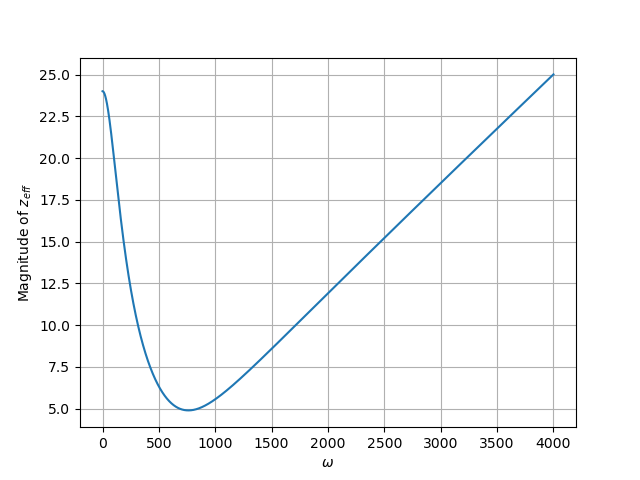
\includegraphics[width = \columnwidth]{2022/IN/52/figs/Zplot.png}
    \caption{Plot of $Z_{\text{eff}}$ vs $\omega$}
    \label{fig:2_gate.22.in.52}
\end{figure}
%\end{document}

\pagebreak

\item A single-phase full-bridge diode rectifier feeds a resistive load of $50 \Omega$ from a 200 V,
50 Hz single phase AC supply. If the diodes are ideal, then the active power, in watts,
drawn by the load is \rule{1cm}{0.5mm} (round off to nearest integer).  \\
\hfill (GATE EE 32)\\
\solution
\iffalse
\documentclass[journal,12pt,twocolumn]{IEEEtran}
\usepackage{amsmath,amssymb,amsfonts,amsthm}
\usepackage{txfonts}
\usepackage{tkz-euclide}
\usepackage{listings}
\usepackage{gvv}
\usepackage[latin1]{inputenc}
\usepackage{adjustbox}
\usepackage{array}
\usepackage{tabularx}
\usepackage{pgf}
\usepackage{lmodern}
\usepackage{circuitikz}
\usepackage{tikz}
\usepackage{graphicx}
\usepackage[english]{babel}

\begin{document}
\bibliographystyle{IEEEtran}

\vspace{3cm}

\title{}
\author{EE23BTECH11047 - Deepakreddy P
}
\maketitle
\newpage
\bigskip

\noindent \textbf{32} \quad A single-phase full-bridge diode rectifier feeds a resistive load of $50 \Omega$ from a 200 V,
50 Hz single phase AC supply. If the diodes are ideal, then the active power, in watts,
drawn by the load is \rule{1cm}{0.5mm} (round off to nearest integer).  \\
\hfill (GATE EE 32)\\
\solution\\
\fi

\begin{figure}[ht]
  \centering
      \begin{circuitikz}[american]
   \draw (0,8) to [sV=200V](0,-1) to [short](6,-1) to [short](6,0) to [D,l=$D_3$](9,3);
   \draw (0,8) to [short](6,8) to [short](6,6);
   \draw (6,6) to [D,l=$D_1$](9,3);
   \draw (3,3) to [D,l=$D_4$](6,6);
   \draw (3,3) to [D,l=$D_2$](6,0);
   \draw (3,3) to [short](2.5,3) to [crossing, bipoles/crossing/size=1](2.5,-4.8) to [short](12,-4.8) to [R=50$\Omega$](12,3) to [short](9,3);
   \draw (9,3) to [short,i=\Large{I}](12,3);
\end{circuitikz}

  \caption{Circuit-1}
\end{figure}

\begin{figure}[ht]
   \centering
   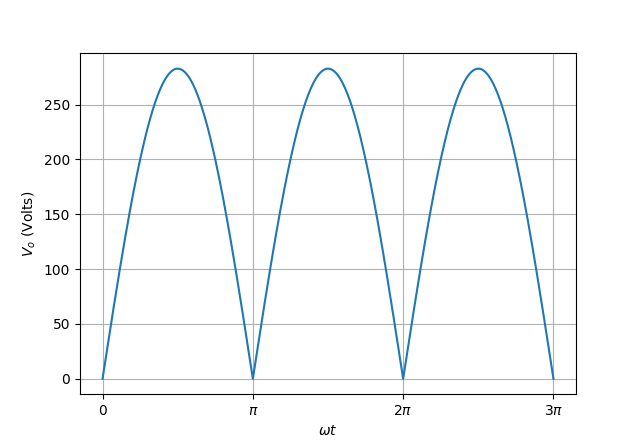
\includegraphics[width=1.2\columnwidth]{2022/EE/32/figs/gt1.png}
   \caption{Output voltage waveform of single-phase full
bridge rectifier}
\end{figure}


\begin{center}
    \begin{table}[ht]
        \setlength{\arrayrulewidth}{0.3mm}
\setlength{\tabcolsep}{12pt}
\renewcommand{\arraystretch}{1.3}


\begin{center}
\caption{Input Parameters}
\begin{tabular}{ |p{1.7cm}|p{1.7cm}|p{1.7cm}|  }

\hline
 {Symbol}&{Description} & {value}\\
\hline
R & Load Resistance & 50$\Omega$\\
\hline
$V_{rms}$ & RMS Voltage  & 200V\\
\hline
f & Frequency & 50Hz \\
\hline

\end{tabular}
\end{center}

    \end{table}
\end{center}

\begin{align}
    V_{rms} &= 200\\
    P &= \frac{\brak{V_{rms}}^2}{R}\\
    P &= \frac{\brak{200}^2}{50}W\\
    P &= 800W
\end{align}


%\end{document}


\pagebreak

\item Let an input $x\brak{t}=2\sin (10\pi t )+5\cos (15\pi t)+7\sin(42\pi t)+4\cos (45\pi t)$ is passed through an LTI system having an impulse response $$h\brak{t}=2\brak{\frac{\sin\brak{10\pi t}}{\pi t}}\cos \brak{40\pi t}$$ The output of the system is \\
\begin{enumerate}[label=(\alph*)]
    \item $2\sin\brak{10\pi t}+5\cos\brak{15\pi t}$
    \item $2\sin\brak{10\pi t}+4\cos\brak{45\pi t}$
    \item $7\sin\brak{42\pi t}+4\cos\brak{45\pi t}$
    \item $5\sin\brak{15\pi t}+7\cos\brak{42\pi t}$
\end{enumerate} \hfill(GATE 2022 EE)\\
\solution
\iffalse
\let\negmedspace\undefined
\let\negthickspace\undefined
\documentclass[journal,12pt,twocolumn]{IEEEtran}
\usepackage{cite}
\usepackage{amsmath,amssymb,amsfonts,amsthm}
\usepackage{algorithmic}
\usepackage{graphicx}
\usepackage{textcomp}
\usepackage{xcolor}
\usepackage{pgfplots}
\usepackage{txfonts}
\usepackage{listings}
\usepackage{enumitem}
\usepackage{mathtools}
\usepackage{gensymb}
\usepackage{comment}
\usepackage[breaklinks=true]{hyperref}
\usepackage{tkz-euclide} 
\usepackage{listings}
\usepackage{gvv}                                        
\def\inputGnumericTable{}                                 
\usepackage[latin1]{inputenc}                                
\usepackage{color}                                            
\usepackage{array}                                            
\usepackage{longtable}                                       
\usepackage{calc}                                             
\usepackage{multirow}                                         
\usepackage{hhline}                                           
\usepackage{ifthen}                                           
\usepackage{lscape}

\newtheorem{theorem}{Theorem}[section]
\newtheorem{problem}{Problem}
\newtheorem{proposition}{Proposition}[section]
\newtheorem{lemma}{Lemma}[section]
\newtheorem{corollary}[theorem]{Corollary}
\newtheorem{example}{Example}[section]
\newtheorem{definition}[problem]{Definition}
\newcommand{\BEQA}{\begin{eqnarray}}
\newcommand{\EEQA}{\end{eqnarray}}
\newcommand{\define}{\stackrel{\triangle}{=}}
\theoremstyle{remark}
\newtheorem{rem}{Remark}
\begin{document}
\parindent 0px
\bibliographystyle{IEEEtran}
\title{GATE: EE - 47.2022}
\author{EE22BTECH11219 - Rada Sai Sujan$^{}$% <-this % stops a space
}
\maketitle
\newpage
\bigskip
\section*{Question}
Let an input $x\brak{t}=2\sin (10\pi t )+5\cos (15\pi t)+7\sin(42\pi t)+4\cos (45\pi t)$ is passed through an LTI system having an impulse response $$h\brak{t}=2\brak{\frac{\sin\brak{10\pi t}}{\pi t}}\cos \brak{40\pi t}$$ The output of the system is \\
\begin{enumerate}[label=(\alph*)]
    \item $2\sin\brak{10\pi t}+5\cos\brak{15\pi t}$
    \item $2\sin\brak{10\pi t}+4\cos\brak{45\pi t}$
    \item $7\sin\brak{42\pi t}+4\cos\brak{45\pi t}$
    \item $5\sin\brak{15\pi t}+7\cos\brak{42\pi t}$
\end{enumerate}
\solution
\fi
\begin{table}[ht]
    \centering
    \begin{tabular}{|p{4cm}|p{2.8cm}|}
    \hline
    Frequency components of input & Value   \\ \hline 
    $$f_1$$ & $$\frac{10\pi}{2\pi}=5Hz$$ \\ \hline
    $$f_2$$ & $$\frac{15\pi}{2\pi}=7.5Hz$$  \\ \hline
    $$f_3$$ & $$\frac{42\pi}{2\pi}=21Hz$$  \\ \hline
    $$f_4$$ & $$\frac{45\pi}{2\pi}=22.5Hz$$    \\ \hline
\end{tabular}

    \caption{Frequency components}
    \label{tab:gate22ee47Q.1}
\end{table}
Given,
\begin{align}
    h\brak{t}&=2\brak{\frac{\sin\brak{10\pi t}}{\pi t}}\cos \brak{40\pi t}  \\
    &=\frac{\sin 50\pi t}{\pi t}-\frac{\sin 30\pi t}{\pi t} \\
    &=h_1\brak{t}-h_2\brak{t}
\end{align}
where,
\begin{align}
    h_1\brak{t} &= \frac{\sin 50\pi t}{\pi t}   \\
    h_2\brak{t} &= \frac{\sin 30\pi t}{\pi t}
\end{align}
Taking Fourier transform of $h\brak{t}$
\begin{align}
    h\brak{t} &\overset{\mathcal{F}}{\longleftrightarrow} H_1\brak{f}-H_2\brak{f}
\end{align}
where,
\begin{align}
    h_1\brak{t} &\overset{\mathcal{F}}{\longleftrightarrow} H_1\brak{f}  \\
    h_2\brak{t} &\overset{\mathcal{F}}{\longleftrightarrow} H_2\brak{f}  
\end{align}
Plotting $H_1\brak{f}$ and $H_2\brak{f}$ we get,    \\
\begin{align}
\begin{tikzpicture}
\begin{axis}[
    axis lines=middle,
    xmin=-40,
    xmax=40,
    ymin=-0.5,
    ymax=1.5,
    xlabel={$f$},
    ylabel={$H_1(f)$},
    xtick={-25,25},
    ytick={0,1},
    ]
    \addplot [blue, thick] coordinates {(-35,0)(-25,0) (-25,1) (25,1) (25,0)(35,0)};
\end{axis}
\end{tikzpicture}   \label{kk:gateee47Q.1} \\
\begin{tikzpicture}
\begin{axis}[
    axis lines=middle,
    xmin=-30,
    xmax=30,
    ymin=-0.5,
    ymax=1.5,
    xlabel={$f$},
    ylabel={$H_2(f)$},
    xtick={-15,15},
    ytick={0,1},
    ]
    \addplot [blue, thick] coordinates {(-25,0)(-15,0) (-15,1) (15,1) (15,0)(25,0)};
\end{axis}
\end{tikzpicture}   \label{kk:gateee47Q.2}
\end{align}
Plotting $H\brak{f}$ from \figref{kk:gateee47Q.1} and \figref{kk:gateee47Q.2}
\begin{tikzpicture}
\begin{axis}[
    axis lines=middle,
    xmin=-40,
    xmax=40,
    ymin=-0.5,
    ymax=3,
    xlabel={$f$},
    ylabel={$H(f)$},
    xtick={-25,-15,15,25},
    ytick={0,1},
    ]
    \addplot [blue, thick] coordinates {(-35,0)(-25,0)(-25,1)(-15,1)(-15,0)(15,0)(15,1)(25,1)(25,0)(35,0)};
\end{axis}
\end{tikzpicture}   \\
Therefore, the given system is a Bandpass filter with passband: \\
\begin{align}
    15\leq\abs{f}\leq 25    \label{equation:gate22ee47Q.1}
\end{align}

Veryfying \tabref{tab:gate22ee47Q.1} with \eqref{equation:gate22ee47Q.1}, only $f_3$ and $f_4$ will be passed through the system. \\
\begin{align}
    \therefore y\brak{t}=7\sin\brak{42\pi t}+4\cos\brak{45\pi t}
\end{align}
($\because\abs{H\brak{f}}=1$, the amplitude of frequency components will be unchanged.)
%\end{document}

\pagebreak

\item In the bandpass filter circuit shown, $R_0 = 50\Omega$, $L_0 = 1 mH$, $C_0 = 10nF$. The q factor of the filter is 
\hfill(GATE 2022 IN 33)
\begin{figure}[h]
\renewcommand\thefigure{1}
    \centering
    \begin{circuitikz}[american]
    \draw (0,0) to [L=$L_0$, *-] (2,0) to [C=$C_0$] (4,0) to [R=$R_0$] (4,-2) to [short, -*] (0,-2);
    \draw (4,-0.3) to[short, -*] (6,-0.3);
    \draw (4,-1.7) to[short, -*] (6,-1.7);

    \node at (6,-1) {Output};
    \node at (0,-1) {Input};
    \end{circuitikz}
    \label{fig:1}
\end{figure}


\solution
\iffalse
\let\negmedspace\undefined
\let\negthickspace\undefined
\documentclass[journal,12pt,twocolumn]{IEEEtran}
\usepackage{cite}
\usepackage{circuitikz}
\usepackage{amsmath,amssymb,amsfonts,amsthm}
\usepackage{algorithmic}
\usepackage{graphicx}
\usepackage{textcomp}
\usepackage{xcolor}
\usepackage{txfonts}
\usepackage{listings}
\usepackage{enumitem}
\usepackage{mathtools}
\usepackage{gensymb}
\usepackage{comment}
\usepackage[breaklinks=true]{hyperref}
\usepackage{tkz-euclide} 
\usepackage{listings}
\usepackage{gvv}                                        
\def\inputGnumericTable{}                                 
\usepackage[latin1]{inputenc}                                
\usepackage{color}                                            
\newtheorem{theorem}{Theorem}[section]
\usepackage{array}                                            
\usepackage{longtable}                                       
\usepackage{calc}                                             
\usepackage{multirow}                                         
\usepackage{hhline}                                           
\usepackage{ifthen}                                           
\usepackage{lscape}
\newtheorem{problem}{Problem}
\newtheorem{proposition}{Proposition}[section]
\newtheorem{lemma}{Lemma}[section]
\newtheorem{corollary}[theorem]{Corollary}
\newtheorem{example}{Example}[section]
\newtheorem{definition}[problem]{Definition}
\newcommand{\BEQA}{\begin{eqnarray}}
\newcommand{\EEQA}{\end{eqnarray}}
\newcommand{\define}{\stackrel{\triangle}{=}}
\theoremstyle{remark}
\newtheorem{rem}{Remark}
\begin{document}
\bibliographystyle{IEEEtran}
\vspace{3cm}
\title{GATE 22 IN/33}
\author{EE23BTECH11040 - Manoj Kumar Ambatipudi$^{*}$% <-this % stops a space
}
\maketitle
\newpage
\bigskip
\renewcommand{\thefigure}{\theenumi}
\renewcommand{\thetable}{\theenumi}
\textbf{QUESTION:}
In the bandpass filter circuit shown, $R_0 = 50\Omega$, $L_0 = 1 mH$, $C_0 = 10nF$. The q factor of the filter is 
\begin{figure}[h]
\renewcommand\thefigure{1}
    \centering
    \begin{circuitikz}[american]
    \draw (0,0) to [L=$L_0$, *-] (2,0) to [C=$C_0$] (4,0) to [R=$R_0$] (4,-2) to [short, -*] (0,-2);
    \draw (4,-0.3) to[short, -*] (6,-0.3);
    \draw (4,-1.7) to[short, -*] (6,-1.7);

    \node at (6,-1) {Output};
    \node at (0,-1) {Input};
    \end{circuitikz}
    \label{fig:1}
\end{figure}


\textbf{SOLUTION:}
\fi
\begin{table}[h]
\renewcommand\thetable{1}
    \centering
    \begin{tabular}{|c|c|c|}
    \hline
     Variable & Description&Value\\\hline
        $R_0$ & Resistance & $50\Omega$ \\\hline
        $L_0$ & Inductance & $1mH$ \\\hline
        $C_0$ & Capacitance & $10nF$\\\hline
        $\omega_0$& Resonant Angular Frequency & $\frac{1}{\sqrt{L_0C_0}}$\\\hline
    \end{tabular}
    \caption{Variables and their description}
    \label{tab_22_33_1}
\end{table}
\\
The corresponding Laplace domain circuit is 
\begin{figure}[h]
\renewcommand\thefigure{2}
    \centering
    \begin{circuitikz}[american]
    \draw (0,0) to [generic=$sL_0$, *-] (2,0) to [generic=$\frac{1}{sC_0}$] (4,0) to [generic=$R_0$] (4,-2) to [short, -*] (0,-2);
    \draw (4,-0.3) to[short, -*] (6,-0.3);
    \draw (4,-1.7) to[short, -*] (6,-1.7);
    \node at (6,-1) {Output};
    \node at (0,-1) {Input};
    \end{circuitikz}
    \label{fig:2}
\end{figure}


Input $X\brak{s}$ can be written as
\begin{align}
    X\brak{s} = I\brak{s}\brak{sL_0 + \frac{1}{sC_0} + R_0} 
\end{align}
Output $Y\brak{s}$ can be written as 
\begin{align}
    Y\brak{s} = I\brak{s}R_0
\end{align}
Transfer function $H\brak{s}$ can be written as 
\begin{align}
    H\brak{s} &= \frac{Y\brak{s}}{X\brak{s}}\\ &= \frac{sC_0R_0}{s^2C_0L_0 + C_0R_0s + 1}
\end{align}
substituting $s = j\omega$
\begin{align}
    H\brak{j,\omega} = \frac{j\omega C_0R_0}{-\omega^2C_0L_0 + jC_0R_0\omega + 1}\\
\implies \abs{H\brak{j,\omega}} = \frac{\omega C_0R_0}{\sqrt{\brak{1-\omega^2C_0L_0}^2 + \brak{C_0R_0\omega}^{2}}}
\end{align}
Differentiating w.r.t $\omega$ and equating to 0, we get 
\begin{align}
    \frac{d\abs{H\brak{j,\omega}}}{d\omega} &= \frac{C_0R_0}{\sqrt{\brak{1-\omega^2C_0L_0}^2 + \brak{C_0R_0\omega}^{2}}} +\notag\\& \frac{\omega C_0R_0}{2\brak{\brak{1-\omega^2C_0L_0}^2 + \brak{C_0R_0\omega}^{2}}^{\frac{3}{2}}}\notag\\&\brak{2\omega\brak{C_0R_0}^2-2\brak{1-\omega^2C_0L_0}2\omega} &= 0\\
    \implies \omega_0 &= \frac{1}{\sqrt{L_0C_0}}\label{eq_22_33_1}
\end{align}
from \tabref{tab_22_33_1}, 
\begin{align}
    \omega_0 = 316227.76
\end{align}
$Q-factor$ defined with reference to inductor
\begin{align}
    Q &= \abs{\frac{V_L}{V_R}}_{\omega_0}\\
      &= \frac{L_0\omega_0}{R_0}\\
      &= \frac{1}{R_0}\sqrt{\frac{L_0}{C_0}} \quad\brak{\text{from \eqref{eq_22_33_1}}}
\end{align}
$Q-factor$ defined with reference to capacitor
\begin{align}
    Q &= \abs{\frac{V_C}{V_R}}_{\omega_0}\\
      &= \frac{1}{C_0\omega_0R_0}\\
      &= \frac{1}{R_0}\sqrt{\frac{L_0}{C_0}} \quad\brak{\text{from \eqref{eq_22_33_1}}}
\end{align}
Substituting the values from \tabref{tab_22_33_1}, we get
\begin{align}
    Q = 200
\end{align}
\begin{figure}
\renewcommand\thefigure{1}
    \centering
    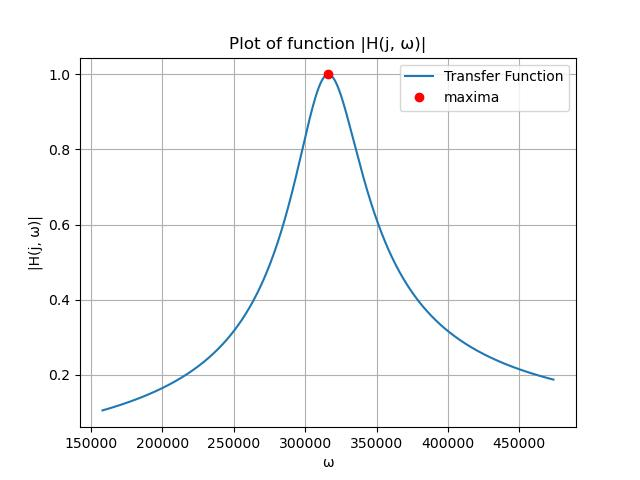
\includegraphics[width=1.0\columnwidth]{2022/IN/33/figs/fig_1.jpg}
    \caption{Transfer function $\abs{H\brak{j, \omega}}$ taken from python3}
    \label{fig:enter-label}
\end{figure}

\pagebreak
\end{enumerate}
